% !TeX root = ../thesis_main.tex

% ---------------------------------------------------
% ----- Chapters of the template
% ----- for Bachelor-, Master thesis and class papers
% ---------------------------------------------------
%  Created by C. Müller-Birn on 2012-08-17, CC-BY-SA 3.0.
%  Freie Universität Berlin, Institute of Computer Science, Human Centered Computing. 
%
% TODO remove 2 - to use auto numbering
\chapter{Implementation and deployment}
\label{chap:impl} 

The phase of implementation and deployment followed an agile development process, where I could deploy changes easily to get fast feedback from users.

% \localtableofcontents

\section{Architecture}

Let's start with an overview about the architecture and high level user flows.
We have three software components relevant for a basic interaction with the system: the UI editor frontend, the UI editor backend and the ''Manager'' backend, which is responsible for
authentification, app management and providing the dynamic resources in an ZIP format.
\\
At the beginning of a user journey, the user visits the root domain (e.g. \url{https://builder.purplemanager.com} for production apps) and logs himself in with username and password.
These credentials are validated in the manager backend, returning an session token which grant's the user access to specific apps he is entitled to see and edit.
Then, he can select one of the available apps he wants to edit.
The following UML sequence diagram displays a typical interaction of a user with the editor frontend after he selected an app; pulling the latest dynamic resourses, editing a file and merging the changes.
\begin{figure}[h]
  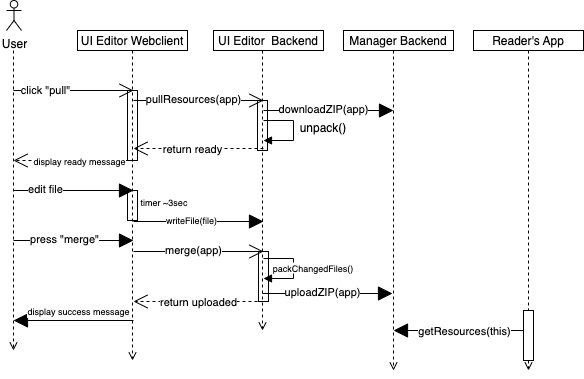
\includegraphics[width=\textwidth]{pics/user-flow.uml.drawio.png}
\end{figure}

\section{Software stack}
From the company's point of view, it is advantageous to keep the technology stack as narrow as possible.
Without restrictions one may chose the latest and greatest language or framework for a new project, but maintainability and availability of persons to review and collaborate are not guaranteed.
For this case study, the most important point was the availability of additional persons with knowledge about the frameworks and languages used. Additional constraints from DevOps'
\footnote{DevOps, short for developer operations, refers to methods or in this case responsible persons to manage the combination of software developemnt and IT operations, e.g. how the code get's deployed, how services get provided and resolved and more.} side were only vague,
since the code gets deployed in Kubernetes, a containerized environment, so the only baisc requirement is that the application must be able to run inside a Docker container.
\\\\
For this project I decided to use Typescript language (\url{https://www.typescriptlang.org}) on both back- and frontend.
The advantages are wide availability of persons in the company who also work with it, a mature ecosystem, and shared type declarations between server and client,
reducing the risk of working with incompatabile data types by accident.
\\
The rest of the stack is fairly common in the web developemnt industry too, the frontend uses React JS as a rendering and reactivity framework,
with additional libraries for state management, UI Components and API query management on top.
\\
For the backend, I used Node as a Javascript runtime, combined with the most used HTTP server framework for Node, Express JS \cite{Github:VanoDevium/node-framework-stars}.
On top of express, a framework called TSOA (\url{https://github.com/lukeautry/tsoa}) is used to improve the developer expeirence. It provides a class based architecture similar
to the well known Spring platform for java, including dependency injection, type validation of the http parameters at runtime and automatic API documentation in the OpenAPI specifications.

Frontend, backend and shared libraries are stored in a monorepo to speed up development and deployments and make refactorings more consistent while maintaining clear APIs and reducing accidental tight coupling.

\section{Feature examples}

In the following section, I'll present a selection of the features that were implemented during the UI editor case study.
These features are chosen as examples to how the HCI methods and outcomes from the user research phase influenced their design and how they can improve the user's experience with the tool. 

(connect to HCI research)
\\
Files:

- multiple tabs as files -> switch between files more fluent, no wait times, discovered during mod. observation

- quick links -> shortcut to often used files, input from interview
\\
Editing

- messages.json custom editor (feedback Anja) -> demo for custom editors per file, 

- changed files -> current implementation, plans to use git as source of truth

- editor abstraction? (more techincal for prechelt for example)
\\
Post processing pipelines


\section{CI/CD}

CI/CD, short for Continous Integration and Continous Deployment, is a core practice of agile software development and provides a log of value to
HCI projects. The first part, Continous Integration, means ''[...] developers add to a shared repository frequently that integrates their code.'' \cite[p. 81]{LearnHCI:2020ys}
The integration consists of automatic builds and tests (cf. \ref*{sec:automated-testing}) to improve quality of the code and confidence of the developers to publish changes more frequently.

As Sprylab uses and private gitlab, for the Expeirence Builder I set up a Gitlab CICD Pipeline. The stages may change when additional build steps or tests are added, but currently it consists of the following stages: \textit{Build}, \textit{Package} and \textit{Deploy}.
\\
\textit{Deploy} is only active on the develop and master Branches and contains the code to upload the docker image to the company's staging and production clusters and update the kubernetes deployment to run the latest build.
The other two stages are run for every Commit of an Merge request. This has the benefit that as soon as a developer pushes his code to a branch that has a Merge Request open,
he and all others can see if the latest commit could be merged safely or if there is more work to do.
The \textit{Build} stage installs the dependencies, builds all packages in the monorepo and executes unit- and e2e-tests afterwards. If any of these steps fail, the Merge request can't be merged until this issue is resolved.

Of course the benefit of CI/CD depends on the setup of the build chain, amount, coverage and quality of tests and other factors. To further improve code quality, we integrated Sonarqube into the repository on gitlab (\url{https://www.sonarqube.org}),
which is a service that automatically scans the code and reports code quality, security issues and technical debt added in a commit.

Having a fast and reliable CI/CD process early on during prototyping and development prooved very valuable, as I could quickly react to user's input on new features or bugs, implement and deploy them quickly on a staging system and get feedback
on the new behaviour in less than 15 minutes. Through the seperation of staging and production system, I could deploy quick fixes with more confidence even when beta testers were working on the production system, as I could verify that my changes
worked in a production-like environment without interrupting users.

\section{Automated Testing}
\label{sec:automated-testing}

As already elaborated, the quality and quantity of automated tests plays a huge role when using CI/CD, as it drastically reduces the time required by Quailty Assurance testers to go through all the edge cases on every change.
For the Experience Builder I stuck to two of the most common testing levels: unit tests and End-to-End tests (also known as E2E or System tests).
\\\\
Unit tests are mostly used to test one ''component'' in an sandboxed environment. For the server, this meant testing Services and classes or even finer grained; single functions.
On the client, we distinguished between UI testing of single react components, and business logic code that is encapsulated in classes or Javascript modules.

They also are helpful during development to test software patterns before dogin large refactorings and to do test-driven development (TDD), where the specifications and constraints can be laid out as code
with invariants, pre- and postconditions, and then the implementation is performed while continously running the tests again until the don't fail anymore.
\\
Espeically for TDD, but also for the CI/CD Pipelines, the speed of the tests is important. If a single test run takes multiple minutes, the developer is blocked during that time and can't progress on the task,
but the duration is also not long enough to start working on another task in the meantime.
That's why I tried to integrate a fast test runtime comatible with UI- / browser testing as well as node runtimes for the server code.
After evaluating diffrent commonly used frameworks, I settled for Vitest (\url{https://vitest.dev/}), which fullfills all the requirements, runs tests in parallel, thus reducing the
time between saving the change and seeing the test result to often less than a second, and has easy integration mechanisms into our build tools.
\\\\
While unit tests are a good way to verify encapsulated behaviours, when many components interact with each other, new errors can emerge often as it is
quite unrealistic to have all intenral and extenral APIs behaving exactly as expected for every input, and Web based UI applications have unmanagable number of factors that
influence the behaviour of UI, network and timings.
\\
E2E tests are supposed to cover a typical user interaction with the service to vaildate the interaction between business logic components, UI and the user itself.
I started with using a custom setup of a headless browser\footnote{Headless browsers are browser instances that don't render the actual content to a user's screen, but run as a CLI application and still execute all Javascript, CSS and HTML.} (\url{https://pptr.dev/}) in combination with vitest,
but writing and especially debugging the tests prooved slow and error prone.
\\
At an internal training day some colleagues introduced a new E2E test framework called Playwright (\url{https://playwright.dev/}), which allows recording a test case in a ''normal'' browser window, it then generates the base code for the test automatically and only needs to be adapted in a few places.
After looking through some examples and seeing how it can get integrated into our pipelines, I started porting the exisitng tests to playwright, and after a few hours the tests run on the new framework, now with much better debugging tools and the ability to add new tests much faster.
\\
This can be an example for others, that investing time to investigate new tools and port code to them if they bring value, can improve developer expeirence and thus also speed and confidence.

\section{Scalability}

- REDIS pubsub + observables
- code example

\section{User Testing, Feedback, Beta and Monitoring}
- deployments to staging
- small test group at start
- internal beta
 - problem: people didn't want to adapt new platform??
- beta flags

\section{Communication and Documentation}

- teams
- jira
- documentation in tool \& external
